% Basic stuff
\documentclass[a4paper]{article}
\usepackage[10pt]{extsizes}

% 3 column landscape layout with fewer margins
\usepackage[landscape, left=0.75cm, top=1cm, right=0.75cm, bottom=1.5cm, footskip=15pt]{geometry}
\usepackage{flowfram}
\ffvadjustfalse
\setlength{\columnsep}{0.01cm}
\Ncolumn[<9]{3}
\onecolumn[9]


% define nice looking boxes
\usepackage[many]{tcolorbox}

% section smaller
\usepackage{sectsty}
\sectionfont{\large}
\subsectionfont{\small}
% a base set, that is then customised
\tcbset {
	base/.style={
		boxrule=0mm,
		leftrule=1mm,
		left=1.75mm,
		arc=0mm, 
		fonttitle=\bfseries, 
		colbacktitle=black!10!white, 
		coltitle=black, 
		toptitle=0.75mm, 
		bottomtitle=0.25mm,
		title={#1}
	}
}

\definecolor{brandblue}{rgb}{0.34, 0.7, 1}
\newtcolorbox{mainbox}[1]{
	colframe=brandblue, 
	base={#1}
}

\newtcolorbox{subbox}[1]{
	colframe=black!20!white,
	base={#1}
}

\usepackage{titlesec}
\titlespacing*{\section}
{0pt}{0ex}{1ex}
\titlespacing*{\subsection}
{0pt}{0ex}{1ex}

% Mathematical typesetting & symbols
\usepackage{amsthm, mathtools, amssymb} 
\usepackage{marvosym, wasysym}
\allowdisplaybreaks

% Tables
\usepackage{tabularx, multirow}
\usepackage{makecell}
\usepackage{booktabs}
\renewcommand*{\arraystretch}{2}

% Make enumerations more compact
\usepackage{enumitem}
\setitemize{itemsep=0pt}
\setenumerate{itemsep=0pt}

% To include sketches & PDFs
\usepackage{graphicx}
\graphicspath{{./summ_img/}}

% For hyperlinks
\usepackage{hyperref}
\hypersetup{
	colorlinks=true
}



\begin{document}
\section{Display and Color}
\subsection{Display Devices and terms}
\textbf{Emissive: } we have electrodes shooting (CRT, FED, LED, OLED), \textbf{non-emissive:} we manipulate light (LCD) 
\noindent
Terms:
\textbf{resolution, viewing angle, pixel density (PPI), brightness, black level, contrast, color gamut, stereopsis (3D), motion parallax, (auto)stereoscopic (1,2), multi-view, (1): circularly polarized glasses, active shutter gl, (2): lenticular lens, parallax barriers, multi-view: 2D, (auto)stereoscopic and how, frame buffer, resolution: \#scan lines, \#pixels per scan line, bits per pixel; color tables, look up tables (LUT), RGB, CMY, HSV, YIQ, CIE, gamuts, alpha channel, double buffering, } 

\section{2D and 3D Maths}
Represent $(x,y)$ as $(\frac{x}{w},\frac{y}{w},w)$ in hom. coordinate rep.,where $w = 1$, 0 for infinite distance.  
\subsection{Transformation matrixes}
Scaling:$\left(
\begin{smallmatrix} a & 0\\
0 & b \end{smallmatrix}\right)$
Rotation:$\left(
\begin{smallmatrix}\cos \theta & -\sin \theta\\
\sin \theta & \cos \theta \end{smallmatrix}\right)$ 
Shear in x: $\left(\begin{smallmatrix} 1 & a\\ 0 & 1 \end{smallmatrix}\right)$
Translation: $\left(\begin{smallmatrix} 1 & 0 & T_x\\ 0 & 1 & T_y\\ 0 & 0 & 1 \end{smallmatrix}\right)$
Rotation about X-axis: $\left( \begin{smallmatrix} 1 & 0 & 0 & 0 \\ 0 & \cos \theta & -\sin \theta & 0 \\ 0 & \sin \theta & \cos \theta & 0 \\ 0 & 0 & 0 & 1 \end{smallmatrix} \right)$, for y and z swap values around such that y and z row and column only have 1 and 0s
Reflect in $y=mx+b$: $\frac{1}{1+m^2}\left(\begin{smallmatrix} 1-m^2 & 2m & -2mb \\ 2m & m^2 -1 & 2b \\ 0 & 0 & 1+m^2   \end{smallmatrix} \right)$. Reflection over XY (change for YZ, XZ): $\left(\begin{smallmatrix} 1 & 0 & 0 & 0\\ 0 & 1 & 0 & 0\\ 0 & 0 & -1 & 0 \\ 0 & 0 & 0 & 1 \end{smallmatrix}\right)$ 

Always use fixed point rule: translate to origin, scale, rotate, shear, translate back to fixed point

\begin{itemize}
	\item Rigid: Translation + rotation (distance preserving)
	\item Similarity: Translation + rotation + uniform scaling (angle preserving)
	\item Affine: Translation + rotation + scaling + shear (parallelism preserving)
\end{itemize}

\section{Hierarchical Modeling }
\begin{itemize}
	\item Render polygons: triangle strip (preferred) and triangle fan (central vertex)
	\item Data structure: vertex set (seq memory access, - duplicated vertices), indexed face set (reuse vertices and compact, - random memory access)
	\item Hierarchical model: hierarchy of objects and its subobjects
	\item Viewworld transformation: Object space $\to$ world space $\to$ eye space: $M_{world2eye}\times M_{obj2world\times P_{obj}}$ 
	\item Modelling glitches: T-join (not touching due to float computations) break into two triangles, overlapping polygons (flipping colors/z fighting) add triangle or turn off depth test  
\end{itemize}

\section{Interactive 3D control}
We can use the mouse for interactive rotation, we need to construct a rotation matrix for that:
\begin{enumerate}
	\item Put the mouse motion vector in XY eye space: (dx, dy, 0)
	\item Axis of rotation perpedicular to the motion vecotr (-dy, dx, 0)
	\item Angle of rotation relative to motion vector length \\ $\sqrt{dx^2 + dy^2}$ 
\end{enumerate}

Make sure to do it from a fixed point.


\section{Camera, Projection, Clipping}
Physical camera models:
\begin{enumerate}
	\item Pin-hole: (+) easy to simulate, everything in focus, (-) need bright scene, everything in focus
	\item Lenscamera: (+) no need for bright scene, not everything in focus, (-) need more programming, not everything in focus
\end{enumerate}

Camera/OpenGL requires objects, viewer and projection

Viewing coordinate transformation:
$Z_v = \frac{P-L}{|P-L|}, X_v = \frac{X \times Z_v}{|V \times Z_V|}, Y_v = Z_v \times X_v$ 
$M = \left[\begin{smallmatrix} x_v^x & x_v^y & x_v^z & 0\\
y_v^x & y_v^y & y_v^z & 0\\ z_v^x & z_v^y & z_v^z & 0 \\
0 & 0 & 0 & 1  \end{smallmatrix} \right] \left[\begin{smallmatrix} 1 & 0 & 0 & -P_x\\ 0 & 1 & 0 & -P_y \\ 0 & 0 & 1 & -P_z \\ 0 & 0 & 0 & 1 \end{smallmatrix} \right] = R\cdot T$ 

\begin{itemize}
	\item Perspective projection: all rays converge at COP
	\item Orthographic projection: all rays are parallel \begin{itemize}
		\item Oblique Projection: DOP not perpendicular to PP \begin{itemize}[leftmargin=0pt]
			\item Cavalier Projection: DOP makes 45d angle with PP, preserves lengths
			\item Cabinet Projection: DOP makes 64.4d angle with PP, foreshorten lines by one-half
		\end{itemize}
		
		\item Orthographic projection: DOP perpedicular to PP \begin{itemize}[leftmargin=0pt]
			\item Orthogonal Projection: DOP align with an axis, implement by throwing away an axis
			\item Axonometric Projection: arb DOP, not parallel to world X, Y, Z-axis. isometric 120d.
		\end{itemize}
		
	\end{itemize}
	
\end{itemize}

$P_{or} = \left[\begin{smallmatrix} \frac{2}{r-l} & 0 & 0 & - \frac{r+l}{r-l}\\ 0 & \frac{2}{t-b} & 0 &-\frac{t+b}{t-b}\\ 0 & 0 & -\frac{2}{f-n} & -\frac{f+n}{f-n}\\ 0 & 0 & 0 & 1\end{smallmatrix}\right] $  $P_{pers} = \left[\begin{smallmatrix} \frac{2n}{r-l} & 0 & \frac{r+l}{r-l} & 0 \\
0 & \frac{2n}{t-b} & \frac{t+b}{t-b} & 0\\
0 & 0 & -\frac{f+n}{f-n} & -\frac{2fn}{f-n}\\
 0 & 0 & -1 & 0
\end{smallmatrix} \right]$ 
Multiply with eye coordinate

\section{Clipping}
\textbf{Goal:} eliminate parts outside the viewing frustum
Clipping Reasons:
\begin{itemize}
	\item Avoid degeneracies
	\item Efficiency
	\item Rasterization is expensive
\end{itemize}
Clipping is taking a part out, culling is taking a whole part out. No difference to final image.

For point (x,y,z) clipping:
Let's have a plane H (A,B,C,D) such that $Ax + By + Cz + D = 0$, assume $D=1$ for now. If $d = H\cdot p = \frac{(A, B, C,D)(a, b, c, 1)}{\sqrt{A^2 + B^2 + C^2}} \geq 0$ inside. 'd' is signed distance.
 Test against each 6 planes, $(0, 0, -1, -near), (0, 0,1,far), (0,d,h,0), \\(0,d,-h,0),(d,0,h,0), (d, 0, -h, 0)$.

For a line segment pq check $H\cdot p, H\cdot q$ clip the part that's outside. Find clipping point by intersecting $L(t) = P_0 + t\cdot (P_1 - P_0)$ with the plane's equation

\subsection{Cohnen Sutherland}
Outcodes:
$\left[\begin{smallmatrix} 1010 & 0010 & 0110 \\ 1000 & 0000 & 0100 \\ 1001 & 0001 & 0101 \end{smallmatrix} \right] $, we have the algorithm:
\begin{enumerate}
	\item Outcode end-point pairs are checked for trivial acceptance
	\item If it can't be trivially accepted, do region check for trivial rejection
	\item If neither, subdivide so that one or both segments can be discard
	\item Repeat until we can trivially accept or reject
\end{enumerate}

\subsection{Polygon Clipping}
Polygon clipping is symmetric, even when convex. When concave is hard. Naive method requires $N\cdot m$ intersections. 

\subsection{Weiler-Atherton Clipping}
\begin{itemize}
	\item Walk around polygon/window boundary CCW
	\item Compute intersection points
	\item Mark where polygons enter and leave clipping window
	\item Keep those that are inside the window
\end{itemize}


\section{Rasterization}
\subsection{Triangles}
\begin{itemize}[leftmargin=0pt]
	\item Scan line coherence: long horizontal stretches of same fill value
	\item Edge coherence: easy to use line agorithm to calculate line's end points
\end{itemize}

\subsection{Flood Fill vs Boundary Fill}
Both need seed x,y and fill color
\begin{itemize}[leftmargin=0pt]
	\item \textbf{Boundary Fill:}  need boundary color, ignore existing 
	\\non-boundary colors, bresenhamp stairstep boundary ok (4C), must have no diagonal gaps in boundary (8C)
	\item \textbf{Flood Fill:}  color at seed pixel, replace seed color, ignores boundary color, fills stairs only (4C), fills diagonally adjacent (8C)
\end{itemize}



\subsection{Anti-aliasing}
Issues with aliasing: jagged profiles, loss of details, disintegrating textures.
Two concepts
\begin{itemize}
	\item Pre-filtering: treat each pixel as an area, compure relative area ratio and mix colours
	\item Post-filtering: combine multiple samples per pixel
\end{itemize}

AA methods:
SSAA: supersampling (render higher resolution then downsample), MSAA: multisampling (easy but hardware dependent), FXAA: fast approximate (find edges and smooth edges), TXAA: specifically to reduce temporal aliasing.

We can also have aliasing in temporal domain (time), so we can use motion blur to fix this.



\section{ Hidden Surface Removal}

Some parts are not visible to us at all, even after clipping since they could be hidden behind something. Methods:
\textbf{Object order:}  consider each 3D obj once, draw pixels and move on, might draw same pixel, e.g. \textit{Z-Buffer} .
\newline
\textbf{Image order:} consider each pixel once, might compute relationships between objects multiple times, e.g. \textit{Ray Casting} 
\newline
\textbf{Sort first}: find some depth-based ordering and draw from back to front, e.g. \textit{Painter's algorithm}
\newline
\textbf{Sort last:} sort implicitly as more information becomes available, e.g. \textit{Z-buffer}    
\textbf{Ray Casting:} for each pixel $p_i$ construct ray from COP through PP at that pixel and into scene, intersect the ray with every object, color the pixel according to the object with closest intersection: $R(t)=(1-t)c + tp_i$ 
\newline
\textbf{Z-buffer:} keep track of depth, if a different pixel is closer replace.  
\textbf{Z-value interpretation: } bilionear interpolation or barycentric coordinates 
\newline
\textbf{Back Face Culling: } given a solid geometry, we can cull polygons facing away from the viewer. Using the normal vector, a polygon is front facing when $N_p \cdot V > 0$. Works completely for single closed convex object, not for multiple obects, not for concave object, usually only as preprocessing step.
\textbf{Potentially Visible Set:} divide scenes into cells, precompute objects that may be visible in each cell. (+) speed up, (-) memory, computing time, dynamic scenes (?) 
\section{Lighting, Material, Shading}
\subsection*{Types of light sources}
\begin{enumerate}
	\item Directional: infinity away, hom. coordinate (X,Y,Z,0), light parallel, easy comp
	\item Point: finite distance, hom. coordinate (X,Y,Z,1), all direct, hard comp, attennuation: dist. dimmer 
	\item Spot: spherical point light, has cutOffAngle, attenuation by deviation from pointing direction
	\item Extended: line or area of light, all points point light sources, realistic, hard computation, has shadow: umbra and penumbra
	\item Environment: (ass.) infinity away, trace reflected aray at each point, looks like texture mapping 
\end{enumerate}

\subsection{Phong Illummination Model}
$I = k_e + k_aI_a + \sum_i f(d_i)I_{li}(k_d(\mathbf{N\cdot L_i})_+ + k_s(\mathbf{V\cdot R}_+^{n_s}))$ 
\begin{enumerate}
	\item $k_e:$ intrinsic shade (self emission), one colour
	\item $k_aI_a:$ ambient reflection coeff, ambient intensity,
	\item $k_d$: diffuse reflection coefficient, $I_l$ intensity of light rouce, $\mathbf{N}$: normal at surface point, $\mathbf{L}$: direction to light source
	\item Light intensity drops off,so we have \\ $f(d)=min(1, \frac{1}{a+bd+cd^2})$ 
	\item $\mathbf{R}:$ reflection angle, $\mathbf{V}$: viewing angle. 
\end{enumerate}
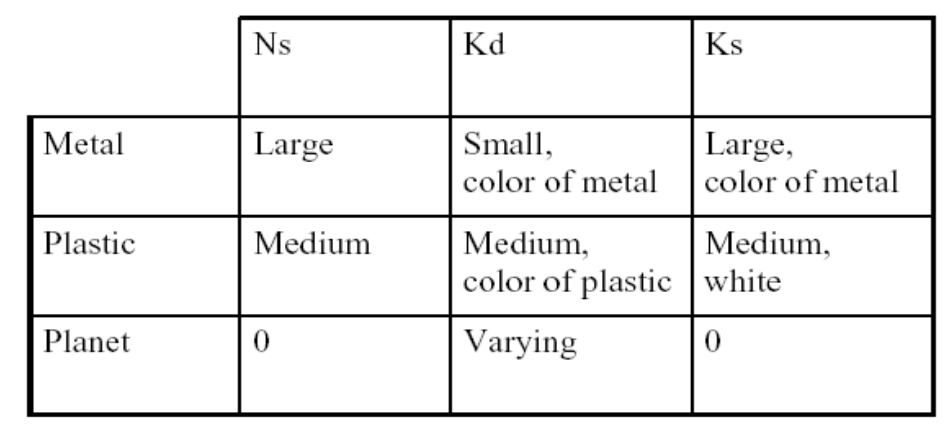
\includegraphics[scale=0.3]{Screenshot_1.png}

\subsection{Interpolative shading}
We want to recover the visual appeareance of a curved surface, we can approximate normals by averaging the normals of all polygons sharing that vertex. The shading can be obtained by a bilinear interpolation or barycentric-coordinate-based interpolation of the approriate quantitties from adjacent vertices

\subsection{Gouraud Shading}
\begin{itemize}
	\item Calculate intensity at each vetex using a local reflection model
	\item Determine by bilinearly interpolating the vertices' intensities
\end{itemize}Issues:
\begin{itemize}
	\item Highlight anomalies: if highlight is in the interior, we may fail to shade it. Solution: smaller polygons
	\item Mach banding: we emphasize intesity changes at a boundary, which creates a banding effect. This can be obvious. Solution: smaller polygons
\end{itemize}

\subsection{Phong Shading}
Solves the interior highlight problem, since we interpolate the vertex normal vectors. This is done at \textbf{each} interior surface point.

Issue in interpolative shading: screen space is not same as world space.

\end{document}
